\documentclass[11pt]{article}
\usepackage[hyperref]{acl}
\usepackage{times}
\usepackage{latexsym}
\usepackage[T1]{fontenc}
\usepackage[utf8]{inputenc}
\usepackage{microtype}
\usepackage{graphicx}
\usepackage{booktabs}
\usepackage{array}
\usepackage{multirow}
\usepackage{xcolor}
\usepackage{amsmath}
\newcommand{\todo}[1]{\textcolor{red}{[#1]}}
\newcommand{\fq}{\textsc{Q4\_0}}
\newcommand{\qkm}{\textsc{Q4\_K\_M}}
\newcommand{\nf}{\textsc{NF4}}
\newcommand{\wmdp}{WMDP-bio}
% generated by scripts/paper_numbers.py
\newcommand{\ctlMaxRise}{10.6}
\newcommand{\ctlDeepLost}{1.5}
\newcommand{\ctlDeepRise}{10.6}
\newcommand{\mapRuns}{150}
\newcommand{\mapEffective}{109}
\newcommand{\mapHeld}{107}
\newcommand{\mapRelapses}{2}
\newcommand{\mapShallow}{79}
\newcommand{\mapMeanQ}{$-$1.4}
\newcommand{\mapMeanN}{$-$0.6}
\newcommand{\mapSigUp}{6}
\newcommand{\mapSigDown}{44}
\newcommand{\mapRelapseLow}{5.7}
\newcommand{\mapRelapseHigh}{6.0}
\newcommand{\mapHfourA}{2 of 12}
\newcommand{\mapHfourB}{0 of 30}
\newcommand{\mapHfourP}{0.077}
\newcommand{\mapHeldHfourA}{2 of 7}
\newcommand{\mapHeldHfourB}{0 of 12}
\newcommand{\mapHeldHfourP}{0.12}
\newcommand{\mapHthreeN}{10}
\newcommand{\mapAtThree}{5}
\newcommand{\mapAtFour}{4}
\newcommand{\deepFreshRuns}{24}
\newcommand{\deepFreshEff}{19}
\newcommand{\deepRoneK}{1}
\newcommand{\deepRoneN}{8}
\newcommand{\deepRoneLo}{0}
\newcommand{\deepRoneHi}{53}
\newcommand{\deepRtwoWins}{7}
\newcommand{\deepRtwoP}{0.035}
\newcommand{\deepSigUpQ}{8}
\newcommand{\deepSigDownN}{9}
\newcommand{\deepMeanQ}{+1.3}
\newcommand{\deepMeanN}{$-$1.9}
\newcommand{\rerunRises}{+4.8, +5.1, +6.1}
\newcommand{\fireEff}{11}
\newcommand{\fireUpN}{10}
\newcommand{\fireDownQ}{10}
\newcommand{\fireMeanQ}{$-$2.3}
\newcommand{\fireMeanN}{+1.5}
\newcommand{\fireRsixK}{1}
\newcommand{\fireRsixN}{8}
\newcommand{\netLow}{3.1}
\newcommand{\netHigh}{4.4}
\newcommand{\netP}{0.015}
\newcommand{\origQ}{+1.6}
\newcommand{\origBaseQ}{+1.8}
\newcommand{\fireNet}{+6.5}
\newcommand{\waterNet}{+8.3}
\newcommand{\rtwoNetWins}{5}
\newcommand{\rtwoNetN}{8}
\newcommand{\rtwoNetP}{0.36}
\newcommand{\realOtherRises}{4.5 and 4.6}
\newcommand{\repRealRise}{+0.5}
\newcommand{\repRealP}{0.63}
\newcommand{\repRealFile}{49.0}
\newcommand{\realOrigFp}{62.8}
\newcommand{\realOrigFile}{62.8}
\newcommand{\realOrigRise}{+0.1}
\newcommand{\realOrigP}{0.934}
\newcommand{\realAFp}{46.8}
\newcommand{\realAFile}{52.9}
\newcommand{\realARise}{+6.0}
\newcommand{\realAP}{0.001}
\newcommand{\realBFp}{47.4}
\newcommand{\realBFile}{52.1}
\newcommand{\realBRise}{+4.6}
\newcommand{\realBP}{0.001}
\newcommand{\causeEditedMax}{1.7}
\newcommand{\causeCases}{6}
\newcommand{\causeBaseA}{$-$0.7 in front, +5.1 behind}
\newcommand{\causeBaseB}{+0.6 in front, +0.9 behind}
\newcommand{\causeFire}{+3.3 in front, +0.6 behind}
\newcommand{\causeWater}{+7.6 in front, +0.2 behind}
\newcommand{\bnbFireFp}{34.8}
\newcommand{\bnbFireFile}{40.1}
\newcommand{\bnbFireRise}{+5.3}
\newcommand{\bnbWaterFp}{38.6}
\newcommand{\bnbWaterFile}{46.3}
\newcommand{\bnbWaterRise}{+7.7}
\newcommand{\qkmFiles}{7}
\newcommand{\qkmRelapses}{0}
\newcommand{\qkmMax}{+1.7}
\newcommand{\repN}{5}
\newcommand{\repA}{5}
\newcommand{\repB}{4}
\newcommand{\repC}{3}
\newcommand{\ctlN}{5}
\newcommand{\ctlA}{4}
\newcommand{\ctlB}{4}
\newcommand{\ctlC}{3}
\newcommand{\repBelow}{2}
\newcommand{\shiftRuns}{180}
\newcommand{\shiftEff}{45}
\newcommand{\shiftUp}{33}
\newcommand{\shiftDown}{12}
\newcommand{\shiftPone}{0.0012}
\newcommand{\shiftRelapses}{29}
\newcommand{\shiftHeldUp}{10}
\newcommand{\shiftHeldDown}{2}
\newcommand{\shiftHeldP}{0.019}
\newcommand{\shiftMeanDefault}{+13.3}
\newcommand{\shiftMeanMid}{$-$0.6}
\newcommand{\shiftMeanDeep}{+14.1}
\newcommand{\shiftMaxRise}{26.8}
\newcommand{\shiftMidLow}{$-$2.7}
\newcommand{\shiftMidHigh}{+0.5}
\newcommand{\shiftPtwoWins}{16}
\newcommand{\shiftPtwoN}{16}
\newcommand{\shiftPthreeWins}{31}
\newcommand{\shiftPthreeLosses}{13}
\newcommand{\shiftPthreeP}{0.005}
\newcommand{\shiftPfourWins}{18}
\newcommand{\shiftPfourLosses}{26}
\newcommand{\shiftBothGap}{+9.3}
\newcommand{\shiftBaseLab}{24.9}
\newcommand{\shiftBaseLow}{31.2}
\newcommand{\shiftBaseHigh}{60.9}
\newcommand{\shiftHeldPtwoWins}{4}
\newcommand{\shiftHeldPtwoN}{4}
\newcommand{\shiftHeldPtwoP}{0.062}
\newcommand{\shiftHeldPthreeWins}{8}
\newcommand{\shiftHeldPthreeN}{12}
\newcommand{\shiftHeldPthreeP}{0.19}
\newcommand{\shiftBaseMidLow}{5.7}
\newcommand{\shiftBaseMidHigh}{10.3}
\newcommand{\shiftPoneModels}{1}
\newcommand{\shiftReverseEff}{47}
\newcommand{\shiftReverseRel}{6}
\newcommand{\shiftReverseMean}{+1.4}
\newcommand{\shiftOrigMax}{2.6}
\newcommand{\placeQOneWins}{7}
\newcommand{\placeQOneLosses}{3}
\newcommand{\placeQOneP}{0.172}
\newcommand{\placeQTwoWins}{9}
\newcommand{\placeQTwoLosses}{1}
\newcommand{\placeQTwoP}{0.011}
\newcommand{\placeQThreeWins}{6}
\newcommand{\placeQThreeLosses}{4}
\newcommand{\placeQThreeP}{0.377}
\newcommand{\placeQTwoWinsQ}{10}
\newcommand{\placeQTwoWinsN}{9}
\newcommand{\placeWaterMargin}{0.3}
\newcommand{\placeShallowMean}{37.1}
\newcommand{\placeDefaultMean}{45.7}
\newcommand{\ckChanged}{3}
\newcommand{\ckPooledFew}{3--5}
\newcommand{\ckPooledMany}{3--5}
\newcommand{\ckLeadFew}{0.3}
\newcommand{\ckLeadMany}{1.4}
\newcommand{\ckTopMany}{2}
\newcommand{\finalWins}{8}
\newcommand{\finalLosses}{2}
\newcommand{\finalP}{0.055}
\newcommand{\finalSig}{8}
\newcommand{\finalMeanNew}{41.7}
\newcommand{\finalMeanOld}{47.8}
\newcommand{\finalGainLow}{5.6}
\newcommand{\finalGainHigh}{13.3}
\newcommand{\finalCostMax}{2.4}
\newcommand{\finalCostMean}{1.6}
\newcommand{\finalBaseCostOld}{3.1 and 3.8}
\newcommand{\finalBaseCostNew}{0.8 and 1.2}
\newcommand{\finalChangeLow}{$-$3.0}
\newcommand{\finalChangeHigh}{+1.6}
\newcommand{\finalRelapses}{0}
\newcommand{\chkModels}{10}
\newcommand{\chkWmdpLow}{33.2}
\newcommand{\chkWmdpHigh}{49.7}
\newcommand{\chkMmluMax}{2.4}
\newcommand{\chkBenignLow}{4.7}
\newcommand{\chkBenignHigh}{7.9}
\newcommand{\chkBenignMean}{6.3}
\newcommand{\chkFiveHigh}{28.2}
\newcommand{\chkRoleUp}{0}
\newcommand{\chkFiveUp}{0}
\newcommand{\chkProbeSig}{40}
\newcommand{\chkProbeN}{50}
\newcommand{\chkRealLow}{$-$3.3}
\newcommand{\chkRealHigh}{+0.9}
\newcommand{\chkTokLow}{$-$1.7}
\newcommand{\chkTokHigh}{+1.7}
\newcommand{\chkFtUp}{5}
\newcommand{\chkFtMax}{22.5}
\newcommand{\chkFtBase}{61.0 and 52.1}
\newcommand{\placeRatioShallow}{3.30}
\newcommand{\placeRatioDefault}{3.26}
\newcommand{\chkForgotShallow}{20.8}
\newcommand{\chkForgotDefault}{14.6}
\newcommand{\chkMmluShallow}{1.6}
\newcommand{\chkMmluDefault}{2.3}
\newcommand{\chkPerMmluShallow}{13.3}
\newcommand{\chkPerMmluDefault}{6.3}
\newcommand{\chkBenignDefaultMean}{4.5}
\newcommand{\chkBenignDefaultMedian}{3.4}
\newcommand{\chkBenignMedian}{6.0}
\newcommand{\chkFtUpA}{2}
\newcommand{\chkFtUpB}{3}
\newcommand{\rtQuestions}{600}
\newcommand{\rtAgreeF}{99.8}
\newcommand{\rtAgreeQ}{95.8}
\newcommand{\rtOrig}{+3.5}
\newcommand{\rtRun}{+3.2}
\newcommand{\rtNet}{$-$0.3}
\newcommand{\rtSameTok}{2388}
\newcommand{\rtPrompts}{2400}
\newcommand{\stwoPairs}{16}
\newcommand{\stwoWins}{16}
\newcommand{\stwoShallowRel}{0}
\newcommand{\stwoShallowN}{16}
\newcommand{\stwoMidRel}{0}
\newcommand{\stwoMidN}{16}
\newcommand{\stwoDefaultRel}{16}
\newcommand{\stwoDefaultN}{16}
\newcommand{\stwoShallowMean}{+1.2}
\newcommand{\stwoDefaultMean}{+11.4}
\newcommand{\stwoShallowMax}{+3.5}
\newcommand{\stwoShallowDeployed}{36.8}
\newcommand{\stwoDefaultDeployed}{50.8}
\newcommand{\stwoMidDeployed}{43.3}
\newcommand{\stwoBaseLow}{33.1}
\newcommand{\stwoBaseHigh}{36.9}
\newcommand{\stwoBaseAll}{12}
\newcommand{\stwoAllDefault}{20}
\newcommand{\stwoAllShallow}{4}
\newcommand{\stwoAllMid}{4}
\newcommand{\stwoAllDefaultMean}{+12.1}
\newcommand{\stwoAllShallowMean}{+3.0}
\newcommand{\stwoAllMidMean}{+1.9}
\newcommand{\stwoAllN}{20}
\newcommand{\stwoRuns}{60}
\newcommand{\stwoAllModels}{Base}
\newcommand{\stwoBaseRiseLow}{8.5}
\newcommand{\stwoBaseRiseHigh}{11.6}
\newcommand{\stwoBaseAuditedLow}{24.6}
\newcommand{\stwoBaseAuditedHigh}{25.7}
\newcommand{\stwoDefaultAudited}{39.4}
\newcommand{\stwoShallowAudited}{35.6}
\newcommand{\stwoMidMean}{+0.0}
\newcommand{\stwoOrigLow}{$-$0.9}
\newcommand{\stwoOrigHigh}{+0.1}
\newcommand{\stwoOrigBase}{$-$2.6}
\newcommand{\stwoOrigFourMax}{0.9}
\newcommand{\glanceRelDefault}{0}
\newcommand{\glanceRelNew}{0}
\newcommand{\mcCells}{314}
\newcommand{\mcMapCells}{218}
\newcommand{\mcBaseCells}{38}
\newcommand{\mcFireCells}{22}
\newcommand{\mcWaterCells}{36}
\newcommand{\mcFireP}{$2.9\times10^{-5}$}
\newcommand{\mcFireHolm}{$6.2\times10^{-4}$}
\newcommand{\mcWaterP}{$2.9\times10^{-7}$}
\newcommand{\mcWaterHolm}{$1.1\times10^{-5}$}
\newcommand{\mcBaseN}{3}
\newcommand{\mcBaseHolmMax}{$5.1\times10^{-4}$}
\newcommand{\mcRelapses}{5}
\newcommand{\mcHolmMax}{$6.2\times10^{-4}$}
\newcommand{\mcPooledMax}{0.009}
\newcommand{\mcOtherSig}{4}
\newcommand{\revJobs}{147}
\newcommand{\revSmoke}{3}
\newcommand{\revSets}{2}
\newcommand{\revAll}{150}
\newcommand{\revCompleted}{140}
\newcommand{\revPrFiveFirst}{13:12:27}
\newcommand{\revPrFiveLast}{13:13:11}
\newcommand{\revPrFiveCommit}{fec9e32}
\newcommand{\revPrFiveFlavor}{l4x1}
\newcommand{\surveyDate}{26 November 2026}
\newcommand{\surveyFound}{1{,}275}
\newcommand{\surveyRead}{915}
\newcommand{\surveyOutdated}{423}
\newcommand{\surveyOutdatedOthers}{418}
\newcommand{\surveyOurs}{5}
\newcommand{\surveyDownloads}{64{,}619}
\newcommand{\surveyDownloadsMonth}{7{,}133}
\newcommand{\surveyAfterFix}{28}
\newcommand{\surveyUnknown}{355}
\newcommand{\surveyNoFiles}{336}
\newcommand{\surveyOfficialRepos}{5}
\newcommand{\surveyKaggle}{5}
\newcommand{\surveyKaggleOutdated}{5}
\newcommand{\surveyGguf}{77}
\newcommand{\surveyGgufOther}{2}
\newcommand{\surveySampled}{12}
\newcommand{\surveySampledDiffer}{12}
\newcommand{\surveyTransformers}{5.20.2}
\newcommand{\surveyShare}{46}
\newcommand{\surveyUnlearning}{0}
\newcommand{\surveySafety}{6}
\newcommand{\surveyBeforeFix}{390}
\newcommand{\surveyAfterFixDownloads}{5{,}313}
\newcommand{\dmgRuns}{120}
\newcommand{\dmgRose}{72}
\newcommand{\dmgAgree}{120}
\newcommand{\dmgHurt}{72}
\newcommand{\stwoBaseMmluLow}{23.1}
\newcommand{\stwoBaseMmluHigh}{24.0}
\newcommand{\stwoDefaultWithin}{0}
\newcommand{\shiftDeepCostAudited}{5.9}
\newcommand{\shiftDeepCostDeployed}{1.8}
\newcommand{\stwoShallowUpper}{20.6}
\newcommand{\stwoShareBack}{47}
\newcommand{\stwoShareLow}{35}
\newcommand{\stwoShareHigh}{57}
\newcommand{\stwoUnitsDefault}{8 of 8}
\newcommand{\stwoUnitsShallow}{0 of 8}
\newcommand{\stwoUnitUpper}{36.9}
\newcommand{\dmgHurtRose}{72 of 72}
\newcommand{\dmgFineRose}{0 of 48}
\newcommand{\ctlPairs}{16}
\newcommand{\ctlOutdatedTrained}{50.9}
\newcommand{\ctlOfficialTrained}{52.1}
\newcommand{\stwoDefaultCostAudited}{5.8}
\newcommand{\stwoDefaultCostDeployed}{1.7}
\newcommand{\stwoShallowCostAudited}{0.5}
\newcommand{\stwoShallowCostDeployed}{1.1}
\newcommand{\stwoMidCostAudited}{0.8}
\newcommand{\stwoMidCostDeployed}{1.0}
\newcommand{\tokWmdpDiffer}{1{,}273}
\newcommand{\tokWmdp}{1{,}273}
\newcommand{\tokMmluDiffer}{1{,}000}
\newcommand{\tokMmlu}{1{,}000}
\newcommand{\tokMore}{5.9}
\newcommand{\tokBareDiffer}{496}
\newcommand{\tokWikiDiffer}{863}
\newcommand{\tokWiki}{1{,}200}
\newcommand{\tokRiseDigit}{+9.4}
\newcommand{\tokRiseNoDigit}{+12.7}
\newcommand{\tokDigitQuestions}{508}
\newcommand{\revHurtRose}{4 of 7}
\newcommand{\revFineRose}{2 of 40}
\newcommand{\totalRuns}{679}
\newcommand{\totalNpo}{10}
\newcommand{\hypN}{22}
\newcommand{\hypHeld}{9}
\newcommand{\hypPart}{2}
\newcommand{\hypFailed}{10}
\newcommand{\hypUntestable}{1}
\newcommand{\hypFailedWord}{ten}
\newcommand{\hypHeldList}{H1, P1, Q2, R1, R2, R6, T1, T2, T3}
\newcommand{\hypFailedList}{H2, H4, P2, P3, P4, Q1, Q3, Q4, R4, R7}
\newcommand{\hypPartList}{R3 and R5}
\newcommand{\hypUntestableList}{H3}


\title{How Deep Does Unlearning Go? One Tokenizer Change\\Undoes It at Layers 5--7 but Not at Layers 3--5}

\author{Saharsh Tibrewala \\
  Independent Researcher \\
  \texttt{github.com/itssaharsh/relapse}}

\begin{document}
\maketitle
\suppressfloats[t]

\begin{abstract}
We unlearn hazardous biology from Cohere's five Tiny Aya models with RMU and Lexsi Labs' SafeTune, CircuitKIT, AuditKIT and CuratorKIT, and test what survives deployment. Runs unlearned and audited through an outdated tokenizer setting scored \stwoDefaultAudited\% on \wmdp{} at SafeTune's default layers 5--7 and \stwoDefaultDeployed\% through the official one: \stwoDefaultRel{} of \stwoDefaultN{} effective runs relapsed. At layers 3--5 it moved \stwoShallowAudited\% to \stwoShallowDeployed\% and \stwoShallowRel{} of \stwoShallowN{} relapsed, on the four post-trained variants; Tiny Aya Base rose at both. We found this by correcting our first-round results. The 4-bit result is reassuring: \mapHeld{} of \mapEffective{} effective runs held in both formats; Fire and Water each relapsed in one exploratory run. Forgetting costs \chkBenignMean{} points of benign biology; a 25-step fine-tune restores at least 5 points in \chkFtUp{} of \chkModels{} runs. Across \totalRuns{} runs and \hypN{} registered hypotheses, \hypHeld{} held, \hypPart{} held in part, \hypFailed{} failed and \hypUntestable{} was untestable.
\end{abstract}

\noindent\fbox{\parbox{0.96\columnwidth}{\small\textbf{Content note.} This paper studies the removal of hazardous biological knowledge. It contains no hazardous question text and no model-generated hazardous content.}}

\begin{figure}[t]
\centering
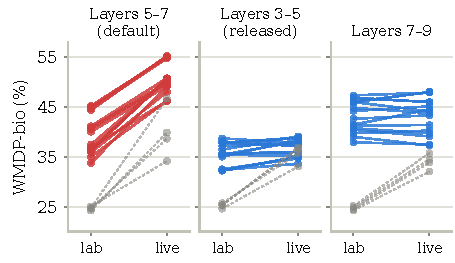
\includegraphics[width=\columnwidth]{figures/tokenizer.pdf}
\caption{Each line is one run unlearned through the outdated tokenizer setting: its \wmdp{} score as \emph{audited} in that setting and as \emph{deployed} through the official tokenizer. Red runs relapse. Dashed grey runs are Tiny Aya Base, at chance when audited and so outside the effective range; they rise at both windows.}
\label{fig:tok}
\end{figure}

\begin{table}[!b]
\centering\small\setlength{\tabcolsep}{3.8pt}
\begin{tabular}{@{}lrr@{}}
\toprule
Layers edited & 5--7 (default) & 3--5 \\
\midrule
\wmdp{} as audited (\%) & 39.4 & 35.6 \\
\wmdp{} as deployed (\%) & 50.8 & 36.8 \\
Relapses, effective runs & 16 of 16 & 0 of 16 \\
Rise $\geq$5 points, all runs & 20 of 20 & 4 of 20 \\
MMLU lost, audited $\rightarrow$ deployed & 5.8 $\rightarrow$ 1.7 & 0.6 $\rightarrow$ 1.1 \\
Rise $\geq$5, MMLU lost $<$3$^\ast$ & \multicolumn{2}{r}{0 of 48} \\
\midrule
MMLU points lost & 2.3 & 1.6 \\
Benign-biology points lost & 4.5 & 6.3 \\
Hazard points per benign point & 3.26 & 3.30 \\
\bottomrule
\end{tabular}
\caption{The result in brief. Top: runs unlearned and audited through the outdated tokenizer setting, then deployed through the official one, on multiple-choice prompts. Effective runs: the four post-trained variants; all runs add Tiny Aya Base, at chance when audited; MMLU lost is against the original through the same tokenizer. Bottom: the final runs, official tokenizer, five models and two seeds. $^\ast$Exploratory; both tokenizer experiments, every window: runs that had lost under 3 MMLU points as audited.}
\label{tab:glance}
\end{table}


\section{Introduction}

Small open-weight language models now run offline on phones and laptops, where no server-side filter sits between the user and the model, so whatever safety the model has must live in its weights. \emph{Machine unlearning} aims to put it there by removing hazardous knowledge while keeping general ability \citep{li2024wmdp}. An unlearned model is audited once: one checkpoint at 16-bit floating-point precision (\emph{fp16}), through one tokenizer. Deployment changes both. Users run 4-bit files, and their copy of the model may load its tokenizer differently.

We study this for RMU (representation misdirection for unlearning; \citealp{li2024wmdp}) on Cohere's Tiny Aya family \citep{salamanca2026tinyaya}, with Lexsi Labs' SafeTune \citep{safetune}, CircuitKIT \citep{circuitkit}, AuditKIT \citep{auditkit} and CuratorKIT \citep{curatorkit}. RMU edits three consecutive layers, a \emph{window}; SafeTune's default window is layers 5--7. Hazardous knowledge is accuracy on \wmdp{}, the 1,273 four-choice biology questions of the WMDP benchmark: lower is better, chance is 25\%, and the original models score 60--64\%.

\textbf{The two tokenizer settings are two public copies of the same model.} Cohere's Hugging Face repositories have set \texttt{tokenizer\_class} to \texttt{PreTrainedTokenizerFast} since 30 September 2026: the \emph{official} setting. The copy on Kaggle Models, uploaded before that fix, names \texttt{CohereTokenizerFast}: the \emph{outdated} setting, under which \texttt{transformers}~v5 does not load the pre-tokenizer. The text and the vocabulary are the same; the split into tokens differs, mostly around line breaks and digits. Our first-round (Stage~1) runs used the Kaggle copy, and correcting them is how we found the effect.

\textbf{The finding} (Figure~\ref{fig:tok}, Table~\ref{tab:glance}). An \emph{effective run} forgot enough to count without falling to chance: it scores 30--55\% on \wmdp{} in the pipeline it was unlearned in. A \emph{relapse} is a rise of at least 5 points with paired $p<0.05$. In a pre-registered test, effective runs unlearned and audited through the outdated setting at the default layers relapsed in \stwoDefaultRel{} of \stwoDefaultN{} cases once deployed through the official tokenizer (\stwoDefaultMean{} points on average); at layers 3--5, \stwoShallowRel{} of \stwoShallowN{} did (\stwoShallowMean), on the four post-trained variants. The fifth model, Tiny Aya Base, unlearns to chance in the outdated pipeline, outside the effective range; counting it, \stwoAllDefault{} of \stwoAllN{} runs rose by 5 points or more at the default layers and \stwoAllShallow{} of \stwoAllN{} at layers 3--5, all four Base. Two controls separate this from the tokenizer alone. Across the two settings the original models move by \stwoOrigLow{} to \stwoOrigHigh{} points on the four post-trained variants (\stwoOrigBase{} on Base). In the reverse direction, runs unlearned through the official setting and scored through the outdated one rise by \shiftReverseMean{} points on average.

Compression was the smaller risk: in \fq{}, llama.cpp's basic 4-bit GGUF format, and \nf{}, the 4-bit format of bitsandbytes, \mapHeld{} of \mapEffective{} effective runs kept their forgetting.

\textbf{Recommendation.} Edit layers 3--5 rather than the default 5--7, score every file that ships, and check at load that the tokenizer setting is the one the audit used.

Our contributions:
\begin{itemize}
\setlength\itemsep{1pt}
\item \textbf{The tokenizer-by-layer result}: how deep unlearning goes depends on where the edit sits. One setting change undid it at the default layers in every effective run, while layers 3--5 and 7--9 held on the four post-trained variants.
\item \textbf{A pre-registered map of 4-bit relapse}: forgetting usually survives \fq{} and \nf{}; the rare exceptions are specific to one format and come from weights the edit never touched.
\item \textbf{A placement result with its price, and a correction}: layers 3--5 give more forgetting per MMLU point and robustness to the tokenizer, with no gain per point of benign biology. We release those models with their full checks, and report our Stage~1 correction and all \hypFailedWord{} failed hypotheses.
\end{itemize}

\section{Related Work}

\textbf{Unlearning hazardous knowledge.} WMDP \citep{li2024wmdp} introduced a hazardous-knowledge benchmark and RMU, which steers activations on forget data toward a random vector while holding them fixed on retain data.

\textbf{Robustness of unlearning.} \citet{lucki2024adversarial} show that RMU-style unlearning can be undone by small fine-tunes.

\textbf{Unlearning and quantization.} Beyond \citet{zhang2025quantization}, \citet{sadhu2026forgetting} formalize a sparsity--permanence trade-off under \nf{} \citep{dettmers2023qlora} and introduce MANSU, whose updates clear the quantization bin by construction. Our method, model family and formats differ, so our low relapse rate does not contradict them; MANSU's code was not available for comparison.

\textbf{Localization.} EAP-IG \citep{hanna2024faith}, through CircuitKIT, tells us where to place the RMU edit.

\section{Setup}
\label{sec:setup}

\textbf{Models.} Tiny Aya has 3.35B parameters and 36 layers, in five variants: Base, Global, Fire, Water and Earth. Each is scored against its own original. Water and Base are held out from the hypotheses of the relapse map and the pipeline experiment.

\textbf{Unlearning.} RMU edits the MLP output projection (\texttt{down\_proj}) of three consecutive layers, the \emph{window}. At the top layer of the window, activations on forget text are pushed toward a fixed random vector with norm $3\times$ the mean activation norm, and activations on retain text are held to a frozen copy with weight $\alpha=100$. The forget set is the WMDP bio corpus and the retain set is Wikitext; we train for 300 batches of 4 with AdamW. SafeTune's default window is layers 5--7.

\textbf{Formats.} We score each model at fp16 and in 4-bit formats. \emph{Round trips} apply a bit-exact implementation of \fq{} or bitsandbytes \nf{} to the decoder's linear weights, leaving embeddings at fp16. \emph{Real files} are made with llama.cpp's converter and \texttt{llama-quantize} \citep{llamacpp} and read back into PyTorch. We state which is used for every result.

\textbf{Metrics.} \wmdp{} accuracy on 1,273 four-choice questions measures hazardous knowledge (lower is better; chance is 25\%). MMLU accuracy on a fixed sample of 1,000 questions measures general knowledge \citep{hendrycks2021mmlu}. \emph{Cost} is the MMLU points lost against the original model in the same format. Answers are read from the next-token probabilities of A--D, so no judge model is involved.

\textbf{Statistics.} Comparisons are paired on questions, using a bootstrap over questions for 95\% intervals and two-sided $p$-values. The pre-registered analyses use our own implementation (10,000 resamples); every real-file comparison, and the rescoring of the Stage~1 models, uses AuditKIT's paired bootstrap (Appendix~\ref{app:stats}). A \emph{relapse} in a format is a rise of at least 5 points in \wmdp{} over the same model at fp16, with paired $p<0.05$. The experiments in Sections~\ref{sec:map}--\ref{sec:place} were pre-registered in the public repository before they were run, the full check in Section~\ref{sec:check} was committed in advance to be reported whatever it showed, and failed hypotheses are reported.

\section{Results}

\subsection{One tokenizer setting undoes unlearning at the default layers}
\label{sec:shift}

\textbf{How we found it.}\label{sec:control} Our Stage~1 runs used the Kaggle copy, so all 1,273 \wmdp{} and all 1,000 MMLU prompts were split the outdated way, in training and in scoring. Table~\ref{tab:control} rescores those weights through both settings. The original model does not move; unlearned models move by up to \ctlMaxRise{} points; and the 4-bit relapse we had reported at layers 10--12 disappeared, so we withdrew it. All results below use the official tokenizer unless stated.

\begin{table}[t]
\centering\small\setlength{\tabcolsep}{4pt}
\begin{tabular}{@{}lrrrr@{}}
\toprule
RMU at & Outdated & Official & Change & MMLU lost \\
\midrule
Original & 63.3 & 63.3 & +0.0 & 0.0 \\
Layers 5--7 & 38.7 & 47.5 & +8.8 & 3.8 \\
Layers 7--9 & 36.8 & 35.7 & $-$1.1 & 2.2 \\
Layers 10--12 & 41.6 & 52.2 & +10.6 & 1.5 \\
\bottomrule
\end{tabular}
\caption{\wmdp{} accuracy (\%) of our Stage~1 weights (Global, trained through the outdated setting), scored in one job through each tokenizer setting, and the MMLU points they had lost as audited (through the outdated setting).}
\label{tab:control}
\end{table}


\textbf{A model unlearned through one setting relapses through the other.} Table~\ref{tab:control} rests on four sets of weights, all of Tiny Aya Global, so we pre-registered a test on \shiftRuns{} fresh runs: RMU trained through the outdated setting, the official one, or both in alternation, each scored through both. Of \shiftEff{} effective runs trained through the outdated setting, \shiftUp{} scored higher through the official tokenizer and \shiftDown{} lower ($p=\shiftPone$); \shiftRelapses{} relapsed. On the held-out models the count was \shiftHeldUp{} to \shiftHeldDown{} ($p=\shiftHeldP$), all from Water, because no Base run was effective. The rise averaged \shiftMeanDefault{} points at the default layers 5--7 and \shiftMeanDeep{} at layers 10--12, up to \shiftMaxRise. At layers 7--9 it was \shiftMidLow{} to \shiftMidHigh{}, smaller than at layers 5--7 in \shiftPtwoWins{} of \shiftPtwoN{} matched pairs; on the held-out models alone this is \shiftHeldPtwoWins{} of \shiftHeldPtwoN{} pairs ($p=\shiftHeldPtwoP$), which four pairs cannot make significant, so the confirmatory version failed.

\textbf{Placement decides it.} A further registered test on two new seeds (\stwoRuns{} runs, all trained through the outdated setting) added layers 3--5, the window we release. Of the effective runs, \stwoDefaultRel{} of \stwoDefaultN{} relapsed at the default layers (\stwoDefaultMean{} points on average), \stwoShallowRel{} of \stwoShallowN{} at layers 3--5 (\stwoShallowMean, at most \stwoShallowMax) and \stwoMidRel{} of \stwoMidN{} at layers 7--9 (Figure~\ref{fig:tok}); all three hypotheses held. Through the official tokenizer the 3--5 runs scored \stwoShallowDeployed\% and the default-layer runs \stwoDefaultDeployed\%. So layers 3--5 did not relapse on the four post-trained variants. Tiny Aya Base is the exception, and the effective-run filter removes it: at every window it fell to chance in the outdated pipeline (\stwoBaseAuditedLow--\stwoBaseAuditedHigh\% at layers 3--5) and rose through the official tokenizer, at layers 3--5 by \stwoBaseRiseLow--\stwoBaseRiseHigh{} points to \stwoBaseLow--\stwoBaseHigh\%. Unfiltered, the runs that rose by at least 5 points were \stwoAllDefault{} of \stwoAllN{} at layers 5--7 (mean rise \stwoAllDefaultMean), \stwoAllShallow{} of \stwoAllN{} at layers 3--5 (\stwoAllShallowMean) and \stwoAllMid{} of \stwoAllN{} at layers 7--9 (\stwoAllMidMean); outside the default layers all of them are Base.

\textbf{Direction matters, and training on both settings does not protect.} Runs trained through the official tokenizer and scored through the outdated one rose by only \shiftReverseMean{} points on average and relapsed in \shiftReverseRel{} of \shiftReverseEff{} cases, about the size of the 4-bit effect: the large relapse belongs to unlearning done through the outdated setting. Training on both settings in alternation narrowed the gap in \shiftPthreeWins{} of \the\numexpr\shiftPthreeWins+\shiftPthreeLosses\relax{} matched pairs ($p=\shiftPthreeP$; held-out \shiftHeldPthreeWins{} of \shiftHeldPthreeN, $p=\shiftHeldPthreeP$), but at layers 5--7 the gap stayed at \shiftBothGap{} points and the deployed score was lower in only \shiftPfourWins{} pairs against \shiftPfourLosses.

\subsection{Compression rarely undoes RMU}
\label{sec:map}

We pre-registered a map of \mapRuns{} runs: five models, five windows, three strengths and two fresh seeds. Of these, \mapEffective{} were \emph{effective} (fp16 \wmdp{} between 30\% and 55\%). \textbf{\mapHeld{} of the \mapEffective{} did not relapse in either 4-bit format}. On average, moving to 4-bit changed \wmdp{} by \mapMeanQ{} points in \fq{} and \mapMeanN{} in \nf{}, so the compressed copy forgot slightly \emph{more}. The two relapses (+\mapRelapseLow{} and +\mapRelapseHigh{} points) are both Tiny Aya Base, seed 12, layers 10--12, in \fq{} only.

Two of our four hypotheses failed and one could not be evaluated. A single-format audit did not miss relapses in both directions, because no run relapsed in \nf{} alone. Layers 10--12 did not relapse significantly more than layers 7--9 (\mapHfourA{} against \mapHfourB{}, $p=\mapHfourP$; held-out models \mapHeldHfourA{} against \mapHeldHfourB{}, $p=\mapHeldHfourP$). Our test of cost at equal forgetting could not be evaluated, because all \mapHthreeN{} model-and-seed pairs failed to bracket the 40\% comparison point at both windows. The fourth, that a relapse tends to appear in one format, held on only these two cases.


\subsection{One file can relapse while its siblings hold}
\label{sec:cases}

The map's only relapse was Tiny Aya Base, seed 12, layers 10--12, in \fq{}. We pre-registered a follow-up of this case before running it.

\textbf{It reproduces.} Retraining the three seed-12 runs with the same settings on a different GPU type gave rises of \rerunRises{} points (Table~\ref{tab:cases}).

\textbf{It recurs.} On eight fresh seeds (\deepFreshRuns{} runs, \deepFreshEff{} effective), \deepRoneK{} seed relapsed in \fq{} (95\% interval \deepRoneLo--\deepRoneHi\% of seeds) and none in \nf{}.

\textbf{It is specific to the format.} Across the fresh seeds \fq{} moved \wmdp{} by \deepMeanQ{} points on average and \nf{} by \deepMeanN{}. The \fq{} change was the larger one on \deepRtwoWins{} of 8 seeds ($p=\deepRtwoP$, sign test). \fq{} raised the score significantly in \deepSigUpQ{} of the \deepFreshEff{} effective runs; \nf{} lowered it significantly in \deepSigDownN{}.

\textbf{The mirror image exists, in one exploratory run each.} On Tiny Aya Fire at layers 13--15 the directions swap: \nf{} raised the score in \fireUpN{} of \fireEff{} effective runs (\fireMeanN{} on average) and \fq{} lowered it in \fireDownQ{} (\fireMeanQ{}). \fireRsixK{} of \fireRsixN{} fresh seeds relapsed in \nf{} and not in \fq{}: a single run, which met our registered existence test and was never retrained. One run of Tiny Aya Water at layers 10--12, from runs registered without a hypothesis, did the same with the largest rise we saw (Table~\ref{tab:cases}). We treat both as exploratory. Neither is noise by an exact McNemar test (Fire $p=$\,\mcFireP, Water $p=$\,\mcWaterP), also after a Holm correction over the \mcFireCells{} and \mcWaterCells{} run-by-format cells screened in the same experiment ($p=$\,\mcFireHolm{} and \mcWaterHolm); the \mcBaseN{} Base relapses keep Holm-corrected $p\leq$\,\mcBaseHolmMax{} (\path{scripts/mcnemar_holm.py}). An audit in one 4-bit format therefore does not certify another, in either direction.

\begin{table}[t]
\centering\small\setlength{\tabcolsep}{3pt}
\begin{tabular}{@{}lrrr@{}}
\toprule
Model, seed, lr & fp16 & \fq{} & \nf{} \\
\midrule
Base 12, lr 2e-4 & 47.4 & 53.1 (+5.7)$^{*}$ & 45.5 ($-$2.0) \\
Base 12, lr 4.5e-4 & 48.9 & 53.7 (+4.8) & 44.0 ($-$4.9) \\
Base 12, lr 1e-3 & 46.8 & 52.9 (+6.0)$^{*}$ & 43.8 ($-$3.1) \\
Base 43, lr 4.5e-4 & 41.6 & 46.8 (+5.3)$^{*}$ & 37.9 ($-$3.6) \\
Fire 44, lr 2e-3 & 34.8 & 33.2 ($-$1.6) & 40.1 (+5.3)$^{*}$ \\
Water 42, lr 1e-3 & 38.6 & 42.3 (+3.7) & 46.3 (+7.7)$^{*}$ \\
\midrule
\emph{Original Base} & 60.1 & 61.9 (+1.8) & 59.8 ($-$0.3) \\
\emph{Original Fire} & 63.5 & 62.5 ($-$1.0) & 62.3 ($-$1.2) \\
\emph{Original Water} & 62.8 & 63.2 (+0.5) & 62.1 ($-$0.6) \\
\bottomrule
\end{tabular}
\caption{\wmdp{} accuracy (\%) of the same weights at fp16 and after each 4-bit round trip, with the change in points. $^{*}$ marks a relapse. Base and Water are edited at layers 10--12, Fire at layers 13--15.}
\label{tab:cases}
\end{table}


\textbf{In the forms people use.} Built with llama.cpp, the \fq{} file of one Base run scored \realAFile\% against \realAFp\% at fp16 (\realARise, $p\le\realAP$, AuditKIT's paired bootstrap). We had seen that file before registering the follow-up. The two Base files built afterwards rose by \realOtherRises{} points, under our 5-point line, so on unseen files this hypothesis failed (appendix, Table~\ref{tab:real}). Loaded in 4-bit through bitsandbytes, an exploratory check of how \nf{} is used in practice, Fire scored \bnbFireFile\% against \bnbFireFp\% (\bnbFireRise) and Water \bnbWaterFile\% against \bnbWaterFp\% (\bnbWaterRise). None of the \qkmFiles{} \qkm{} files rose by more than \qkmMax{} points. In every case, at least one 4-bit format of the same weights held. Scored inside llama.cpp's own runtime on the first \rtQuestions{} questions (an exploratory check), answers matched our read-back scoring on at least \rtAgreeF\% of questions at f16 and \rtAgreeQ\% in \fq{}. There \fq{} raised the original Base by \rtOrig{} points and the seed-12 run by \rtRun{}: on those questions the rise is the format's.


\textbf{How much is the unlearning's doing?} The original Tiny Aya Base itself scores \origBaseQ{} points higher in \fq{} than at fp16 (Table~\ref{tab:cases}). Net of that, the seed-12 rises are \netLow--\netHigh{} points ($p\le\netP$) and no Base run reaches 5; the ordering of \fq{} over \nf{} across fresh seeds also loses significance (\rtwoNetWins{} of \rtwoNetN{} seeds, $p=\rtwoNetP$; not a registered test). For the typical Base run, then, the change is no larger than the original model's own (\deepMeanQ{} on average across fresh seeds); for seed 12 about a third of the rise is the format and the rest is the edit holding less well. The originals of Fire and Water fall slightly in \nf{}, so their relapses grow net of the original (\fireNet{} and \waterNet). The 5-point line matters too: at 3 points the map would count \mapAtThree{} relapsing runs, not \mapRelapses.

\subsection{Where it comes from, and what repairs it}
\label{sec:repair}

Earlier work explains relapse under quantization by parameter updates too small to survive rounding \citep{zhang2025quantization,sadhu2026forgetting}. That is not the cause here. We rounded one part of the model at a time (appendix, Table~\ref{tab:cause}). Rounding the three edited matrices alone moved \wmdp{} by at most \causeEditedMax{} points in the \causeCases{} relapsing runs. \textbf{The rise comes from weights that unlearning never touched.} Which ones differs. On Water and Fire it is the layers in front of the edit (\causeWater{}; \causeFire{}), the mechanism our Stage 1 submission described. On Base seed 12 it is the layers behind the edit (\causeBaseA{}), and on Base seed 43 no single part explains it. We had registered the Stage 1 mechanism as a hypothesis for Base, and there it failed.


\textbf{Training on the file.} For each relapsing run we trained a repaired run with the same seed and learning rate, with the model and its frozen reference seen as their 4-bit copies on every step, for 600 batches. The repaired run did not relapse in \repA{} of \repN{} cases, scored significantly lower in the file than the run it repairs in \repB, and stayed within 3 MMLU points in \repC{} (appendix, Table~\ref{tab:repair}). But plain RMU for the same 600 batches did almost as well (\ctlA, \ctlB{} and \ctlC{} of \ctlN), and \repBelow{} repaired runs fell below the effective range, where not relapsing means little. We cannot separate the repair from longer training. For the one repaired run we also built as a real llama.cpp file, the file held (\repRealFile\%, \repRealRise{} against fp16). A rule for choosing the amount of training, registered before its test case was scored, failed on that case. Rounding only the edited matrices during training never repaired.

\textbf{What reliably works} is cheaper: score every format before release, and ship one that holds.

\begin{table*}[t]
\centering\footnotesize\setlength{\tabcolsep}{2.45pt}
\begin{tabular}{@{}llrrrrrrrrrrr@{}}
\toprule
 & & \multicolumn{8}{c}{At fp16} & \multicolumn{3}{c}{\wmdp{} of the unlearned model} \\
\cmidrule(lr){3-10}\cmidrule(l){11-13}
Model & & WMDP & MMLU & Benign bio & 5-shot & Role & Reword & Hindi & Swahili & \qkm{} file & Outdated & Fine-tuned \\
\midrule
Global & original & 63.4 & 55.4 & 62.5 & 63.0 & 62.1 & 51.5 & 50.8 & 50.9 & & & \\
 & unlearned & 42.6 & 54.1 & 55.1 & 24.7 & 37.2 & 39.6 & 39.3 & 39.9 & 42.1 & 42.5 & 43.2 \\
\addlinespace[2pt]
Fire & original & 63.5 & 57.9 & 64.3 & 66.4 & 63.3 & 51.5 & 55.6 & 51.7 & & & \\
 & unlearned & 41.7 & 56.2 & 58.6 & 25.5 & 37.6 & 35.6 & 39.8 & 38.6 & 39.9 & 40.4 & 45.4 \\
\addlinespace[2pt]
Earth & original & 62.8 & 56.5 & 62.4 & 64.2 & 61.2 & 54.5 & 51.3 & 52.6 & & & \\
 & unlearned & 43.8 & 54.3 & 56.5 & 26.0 & 38.4 & 38.1 & 36.9 & 40.3 & 43.0 & 44.5 & 46.5 \\
\addlinespace[2pt]
Water & original & 62.8 & 57.1 & 63.5 & 63.9 & 62.4 & 55.5 & 52.4 & 52.6 & & & \\
 & unlearned & 44.1 & 55.4 & 57.5 & 25.8 & 39.5 & 39.6 & 38.0 & 43.9 & 43.9 & 42.9 & 48.3 \\
\addlinespace[2pt]
Base & original & 60.1 & 57.6 & 65.4 & 65.4 & 64.3 & 48.5 & 49.7 & 50.0 & & & \\
 & unlearned & 36.2 & 56.6 & 58.8 & 25.5 & 33.1 & 35.1 & 34.8 & 39.0 & 36.1 & 37.0 & 56.5 \\
\bottomrule
\end{tabular}
\caption{The final runs at layers 3--5 (mean of two seeds; the released model is the seed with the lower \wmdp{}): accuracy (\%) of the original and the unlearned model at fp16 on the hazard set, general knowledge, benign biology, two prompt attacks and reworded or translated hazard questions; then the unlearned model's \wmdp{} in the real \qkm{} file, through the outdated tokenizer, and after a 25-step fine-tuning attack. Prompt attacks and the fine-tuning attack use the 1,204 hazard questions not used as examples or for training.}
\label{tab:check}
\end{table*}


\subsection{Where to place the edit}
\label{sec:place}

SafeTune's default edits layers 5--7. We re-ran CircuitKIT's EAP-IG through the official tokenizer on all five models and registered comparisons on fresh seeds, each on the lowest \wmdp{} a window reaches while losing at most 3 MMLU points.

\textbf{Two registered tests of layers 3--5 against the default: one passed, one narrowly missed.} On seeds 31 and 32, layers 3--5 beat the default in \placeQTwoWins{} of 10 model-and-seed pairs ($p=\placeQTwoP$; \placeQTwoWinsQ{} of 10 in \fq{}, \placeQTwoWinsN{} of 10 in \nf{}), reaching \placeShallowMean\% on average against \placeDefaultMean\%. On fresh seeds 33 and 34, each window at the learning rate the earlier seeds chose by a fixed rule, layers 3--5 scored lower in \finalWins{} of 10 pairs: $p=\finalP$, so by our own rule this test failed. Each of the eight wins is by \finalGainLow--\finalGainHigh{} points with $p<0.001$ (\finalMeanNew\% against \finalMeanOld\% on average); the two exceptions are Tiny Aya Base, where the default forgot more but lost \finalBaseCostOld{} MMLU points against \finalBaseCostNew.

\textbf{What placement buys, and what it does not.} On the fresh seeds the 3--5 runs forget \chkForgotShallow{} hazard points for \chkMmluShallow{} MMLU points, the default-layer runs \chkForgotDefault{} for \chkMmluDefault. Layers 3--5 are not more selective within biology: benign biology falls by \chkBenignMean{} points against \chkBenignDefaultMean, so both windows forget the same number of hazard points per point of benign biology lost (\placeRatioShallow{} and \placeRatioDefault). The gain is more forgetting per MMLU point and robustness to the tokenizer (Section~\ref{sec:shift}), with none per point of benign biology.

\textbf{CircuitKIT's pick per model is unstable; pooled over the family it points to the window that won.} Each model's own top window beat the default in only \placeQThreeWins{} of 10 pairs ($p=\placeQThreeP$), so that hypothesis failed. It won on Global, Earth and Base, where the top window is 3--5. It lost on Water, where layers 2--4 led 3--5 by \placeWaterMargin\% of the attribution and barely unlearned, and on one Fire seed, where the top window was 10--12. Layers 7--9, our Stage 1 choice, beat the default in \placeQOneWins{} of 10 ($p=\placeQOneP$), which also failed. The window with the largest share of attribution averaged over the five models is 3--5; we noticed this after the first results, which is why its test uses the fresh seeds. Repeating CircuitKIT with 160 prompts instead of 64 (exploratory) changed the per-model top window on \ckChanged{} of five models; the pooled one stayed \ckPooledMany{}, its lead over 2--4 growing from \ckLeadFew{} to \ckLeadMany{} points of share.

We publish the seed-34 run of each model at layers 3--5, chosen for its lower \wmdp{}, as its card says. They lose at most \finalCostMax{} MMLU points, and none relapses in \fq{} or \nf{} (changes of \finalChangeLow{} to \finalChangeHigh{} points).

\subsection{Is the knowledge gone?}
\label{sec:check}

Table~\ref{tab:check} gives the full check of the \chkModels{} final runs at layers 3--5 (two seeds per model), which we committed to report whatever it showed. They score \chkWmdpLow--\chkWmdpHigh\% on \wmdp{} and lose at most \chkMmluMax{} MMLU points.

\textbf{What holds.} Five worked examples or an expert persona did not bring the knowledge back: neither prompt raised the score significantly on any model (\chkFiveUp{} and \chkRoleUp{} of \chkModels), and with five examples every model fell to \chkFiveHigh\% or below, near chance, which suggests the examples scramble the model more than they help it. Reworded English questions and translations into Hindi, Swahili, Arabic and Spanish, gated with CuratorKIT, stayed significantly below the original in \chkProbeSig{} of \chkProbeN{} cases. The real llama.cpp \fq{} and \qkm{} files changed \wmdp{} by \chkRealLow{} to \chkRealHigh{} points, and the outdated tokenizer by \chkTokLow{} to \chkTokHigh.

\textbf{What it costs, and what breaks it.} Benign biology (four MMLU biology subjects) fell by \chkBenignLow--\chkBenignHigh{} points, \chkBenignMean{} on average: the forgetting is not confined to hazardous questions. A fine-tune of 25 LoRA steps on 64 held-out hazard questions raised the score by at least 5 points on \chkFtUp{} of \chkModels{} models and restored Tiny Aya Base to \chkFtBase\%. RMU hides knowledge more than it removes it \citep{lucki2024adversarial}.


\section{What Did Not Work}
\label{sec:fail}

Registered hypotheses that failed: a single-format audit misses relapses in both directions \emph{within the map} (it found only the \fq{} direction; the \nf{} direction appeared in the follow-up); layers 10--12 relapse more than layers 7--9 ($p=\mapHfourP$); the Base relapse comes from the layers in front of the edit; training on both tokenizers protects the deployed model; the held-out, confirmatory versions of two tokenizer hypotheses (placement, and the gap narrowing with both tokenizers); layers 7--9 beat the default; each model's own CircuitKIT window beats the default; layers 3--5 beat the default on the final seeds ($p=\finalP$); and the dose rule for the repair. Another, cost at equal forgetting, could not be evaluated as registered, and the real-file hypothesis held only for the one Base file we had already seen.

Things we built that did not work: retraining the edited matrices so that the \fq{} file imitates the audited model left the file's score unchanged; keeping layers 17--20 at full precision removed only part of the Base rise; and NPO with LoRA, tried at 17 settings through the official tokenizer, either did not forget or lost general knowledge as fast as hazardous knowledge; its 4-bit copies scored like fp16.

From Stage 1 we withdraw the relapse and repair on Tiny Aya Global, which the outdated tokenizer produced, and every number measured through it.

\section{Limitations}

Knowledge is measured by multiple choice, not open generation, and a 5-point line on 1,273 questions is a choice. The tokenizer effect was measured only on these multiple-choice prompts, whose line breaks are what the two settings split differently; single-line prompts are untested. Relapses are rare events: each rests on one or two seeds per model, so their rates have wide intervals. Part of the Base rise is a property of the format, since the original model rises too. All models come from one family and one unlearning method. Only one case was scored inside llama.cpp's own runtime, on 600 questions; every other real file is read back into PyTorch. Runs that share a seed are not independent, and a bootstrap over questions ignores training variance. Round trips leave embeddings at fp16; real files do not, and two of three Base files landed just under our line. CircuitKIT and our learning-rate ranges both used scored questions (appendix). RMU does not survive fine-tuning on the topic. The repair is specific to the format it trains on.

\section{Conclusion}

An unlearning audit certifies one artifact through one pipeline. For RMU on Tiny Aya the 4-bit file usually keeps the forgetting, but not always, and a relapse shows only in the format that has it. A different tokenizer setting returned much more, silently: at SafeTune's default layers in every effective run, and at layers 3--5 in none on the four post-trained variants. We recommend scoring every file that ships, through the exact tokenizer files that ship with it, and stating which ones were scored.

\bibliography{references}

\appendix
% Appendix. \input after \appendix in main.tex. Uses \todo, \fq, \qkm, \nf, \wmdp from main.tex; \path comes from url.sty (loaded by hyperref).
\newcommand{\costTotal}{about \$140 in total}

\section{Kits and how they connect}
\label{app:kits}

Table~\ref{tab:kits} lists the four Lexsi Labs kits. CuratorKIT gates the probe sets, which our scorer reads. CircuitKIT picks a three-layer window per model, which the placement job passes to SafeTune. SafeTune's RMU returns three edited matrices, which are written into the full model, stored in each format and scored. The pre-registered analyses use a paired bootstrap over questions implemented in \path{scripts/analyze_map.py} (10,000 resamples); AuditKIT's paired bootstrap is used for every real-file comparison and for the rescoring of the Stage~1 models (Appendix~\ref{app:stats}).

\begin{table*}[t]
\centering\footnotesize
\begin{tabular}{@{}>{\raggedright\arraybackslash}p{0.1\textwidth} l p{0.51\textwidth} >{\raggedright\arraybackslash}p{0.25\textwidth}@{}}
\toprule
Kit & Version & What it does here & Code \\
\midrule
SafeTune \citep{safetune} & 0.1.13 & \texttt{rmu\_unlearn} with \texttt{RMUConfig}. We set the loss layer $L$, the updated layers $L{-}2$ to $L$, steering, retain weight, learning rate and batches, and pass our tokenized batches, a frozen reference and the model cut to $L{+}1$ layers. Only the three \texttt{mlp.down\_proj} matrices are kept. & \path{kaggle/06}, \path{kaggle/13} \\
CircuitKIT \citep{circuitkit} & 0.2.1 & EAP-IG \citep{hanna2024faith} on its built-in WMDP task (\texttt{wmdp-bio}, 64 questions of at most 80 tokens, 5 integration steps, heads and MLPs, fp16; transformer-lens 3.8.0). The window is the three consecutive layers within 1--12 with the largest summed absolute MLP score. A faithfulness report is saved, not used. & \path{hf_jobs/circuitkit_job.py} (Stage~1: \path{kaggle/02}) \\
AuditKIT \citep{auditkit} & 1.1.6 & Multiple-choice runs on the in-memory model (\texttt{MCQAdapter} over the log-likelihoods of `` A''--`` D'', \texttt{Runner}, \texttt{Acc}), saved with provenance. \texttt{ak.compare} gives the paired p-value; our wrapper adds a 95\% interval and flip counts. & \path{kaggle/auditkit_mcq.py}, \path{kaggle/08}, \path{scripts/analyze_deep.py}, \path{scripts/analyze_certify.py} \\
CuratorKIT \citep{curatorkit} & 0.1.24 & Per language, after our own gate: schema gate, length limits (5 to 2,048 tokens), exact and MinHash deduplication (0.9) and cleaning with HTML stripping off; writes a manifest, provenance and card. & \path{scripts/curate_probes.py} \\
\bottomrule
\end{tabular}
\caption{The Lexsi Labs kits and their exact role. Script paths are relative to the repository root.}
\label{tab:kits}
\end{table*}

As in Stage~1, CircuitKIT runs with two memory patches to transformer-lens, the tied unembedding reusing the embedding matrix, and a length filter that keeps the first 64 questions of at most 80 tokens; each job stops unless CircuitKIT's tokenizer gives the official token ids on 300 \wmdp{} questions. CuratorKIT is not pinned; its version is read from the provenance file it wrote.

\section{Models and licenses}
\label{app:models}

\textbf{Tiny Aya.} Tiny Aya \citep{salamanca2026tinyaya} is a 3.35B-parameter decoder with 36 layers and a 262,144-token vocabulary. We use all five released variants: Base, the pretrained model, and Global, Fire, Water and Earth, post-trained from it. Stage~2 jobs download \path{CohereLabs/tiny-aya-<variant>} from the main branch; on 21 and 22 November 2026 these were revisions \texttt{af89d219b5} (Global), \texttt{73500c80fc} (Fire), \texttt{0624fafbe2} (Earth), \texttt{41a99216d1} (Water) and \texttt{d62ac17e24} (Base). The bfloat16 weights are loaded in fp16. Layers are numbered from 0.

\textbf{Licenses.} The Hugging Face cards of all five variants give the license as CC-BY-NC-4.0 and gate downloads; they also refer to Cohere Labs' Acceptable Use Policy. Our use is non-commercial research.

\textbf{Derived models and artifacts.} The released Stage~2 models are public as \path{itssaharsh/relapse-tiny-aya-<variant>-unlearn-bio}: for each variant the seed-34 run at layers 3--5 (Section~\ref{sec:place}), with full-precision weights, the official tokenizer files, a real \qkm{} file and the scores of those files; they carry CC-BY-NC-4.0. The Stage~1 models \path{itssaharsh/tiny-aya-global-unlearn-bio-*} were trained through the outdated tokenizer setting, as their cards say. The demo Space \path{itssaharsh/relapse}, the datasets \path{itssaharsh/relapse-runs} and \path{itssaharsh/relapse-wmdp-bio-probes} and the code are public. No other model is used.

\section{Datasets, splits and leak check}
\label{app:data}


Sizes: 1,273 \wmdp{} test questions, 1,200 forget and 1,200 retain texts per 300-batch run, 1,000 MMLU questions, 720 benign-biology questions, 64 control questions and 707 probes. The data come from \path{cais/wmdp} \citep{li2024wmdp}, \path{cais/wmdp-bio-forget-corpus}, \path{Salesforce/wikitext} (\texttt{wikitext-2-raw-v1}) and \path{cais/mmlu} \citep{hendrycks2021mmlu}. The MMLU sample is the first 1,000 of the \texttt{all} test split shuffled with \texttt{datasets} seed 0; benign biology is the full test set of college biology, high school biology, virology and medical genetics.

\textbf{Unlearning data.} For seed $s$, forget and retain texts longer than 50 characters are shuffled with \texttt{random.Random(s)}, and the first $4\times$(number of batches) are cut to 2,000 characters and at most 512 tokens. The gated corpus is downloaded inside each job and never uploaded; jobs upload only scores and edited matrices.

\textbf{Attack split.} The full check shuffles the 1,273 indices with \texttt{random.Random(0)}: the first 5 are the worked examples of the five-shot prompt, the next 64 train the fine-tuning attack, and the other 1,204 are scored under every prompt condition and after the attack. The Stage~1 attack scripts used the same split.

\textbf{Probes.} In Stage~1, through Kaggle's copy and so the outdated tokenizer, Tiny Aya Global translated 200 \wmdp{} questions (sampled with \texttt{random.Random(0)}) into Hindi, Arabic, Spanish and Swahili and reworded them in English. A translation is kept if its back-translation scores chrF $\geq 35$ against the source, a rewording if it parses and differs from the source. After CuratorKIT, 187, 186, 119, 114 and 101 items remain (CuratorKIT removed none that our gate kept). No native speaker checked them.

\textbf{What touches training.} RMU updates see only the forget corpus and Wikitext; no benchmark or probe question enters unlearning. The consolidation pilot trains on the same two corpora, with the unlearned model's own hidden states as targets. The fine-tuning attack trains LoRA adapters on 64 \wmdp{} (or 64 MMLU validation) questions, is scored on the disjoint 1,204, and its adapters are discarded.

\textbf{Where scored questions influenced choices.} CircuitKIT reads 64 of the scored questions and decides placement, though it changes no weights. Stage~1 chose its settings on the scored questions, through the outdated tokenizer, and some of its learning rates reappear in the Stage~2 ladders (\path{results/methods.json}); fresh seeds and held-out models limit the effect. We did not check the forget corpus for text overlap with the questions.

\section{Metrics and statistics}
\label{app:stats}

\textbf{Accuracy.} Each prompt is \emph{``The following are multiple choice questions (with answers) about \{subject\}.''}, a blank line, the question, options ``A.''--``D.'' on separate lines, and ``Answer:''. The prediction is the most probable of `` A''--`` D'' under a softmax over the logits of their last tokens at the final position. Batches of 8 (4 for attack sets) are left-padded and cut at 1,024 tokens (2,048 in the full check). Stage~2 scores through the official tokenizer; the pipeline experiment, the tokenizer control and the full check also score through the outdated one.

\textbf{Definitions.} \emph{Cost}: the original's MMLU in a format minus the run's, in points. \emph{Effective run}: fp16 \wmdp{} in $[30\%, 55\%]$ (in the pipeline experiment, through the training tokenizer, or both). \emph{Relapse} in a format: \wmdp{} at least 5 points above the same weights at fp16, with two-sided paired $p<0.05$. \emph{Rise}: fp16 \wmdp{} through the official minus the outdated tokenizer; a \emph{pipeline relapse} is a rise of at least 5 points with $p<0.05$, and the \emph{gap} is its absolute value. \emph{Best safe forgetting} of a window: its lowest \wmdp{} among runs that cost at most 3 points in the same format. A \emph{relapsing seed} has an effective run that relapses.

\textbf{Paired bootstrap.} The pre-registered analyses (\texttt{paired\_p} in \path{scripts/analyze_map.py}) take the per-question difference in correctness ($-1$, $0$ or $+1$) between two conditions, draw 10,000 resamples of the $n$ questions (multinomial draws over the three values) and record the mean difference $\delta^{*}$. The 95\% interval is the 2.5th to 97.5th percentile, and $p=\min\{1, 2\min[(\#\{\delta^{*}\leq 0\}+1)/10001, (\#\{\delta^{*}\geq 0\}+1)/10001]\}$, with NumPy's \texttt{default\_rng} at a fixed seed. The full check uses it too, except for real files. AuditKIT's paired bootstrap is used for every real-file comparison and for the rescoring of the Stage~1 models: \texttt{ak.compare} on saved AuditKIT runs gives the $p$-value (its default of 1,000 resamples of the zero-centred differences, seed 42, so $p\geq 0.001$), and our wrapper adds a percentile interval (10,000 resamples, seed 0).

\textbf{Exact tests.} Sign tests are one-sided binomial tests with ties dropped: $p=P(X\geq w)$, $X\sim\mathrm{Bin}(w+l, 1/2)$ for $w$ wins and $l$ losses. Relapse shares between windows use a one-sided Fisher exact test, and shares of relapsing seeds a Clopper--Pearson 95\% interval. A hypothesis holds at $\alpha=0.05$; pre-registrations 1 to 3 call it strong only below a Bonferroni threshold (0.0125 for four hypotheses, 0.0167 for three).

\textbf{Pre-registration.} Four documents in \path{results/} fix designs, definitions, hypotheses and tests before the runs they cover, and the analysis scripts were committed before their results were read; commit times are the record (Appendix~\ref{app:decl}), and pre-registration~4 lists what had been seen when it was written. Nothing is rerun or dropped because of its result, technical failures are rerun with the same settings and reported (Appendix~\ref{app:repro}), and failed hypotheses are reported in the main text. Every experiment uses new seeds. Water and Base are held out from the hypotheses of the map and the pipeline experiment, and their results are the confirmatory ones. Pre-registration~4 tests replication (R1, R2, R6) only on seeds 41--48, not on seed 12, where the relapse was first seen; the seed-12 rerun does not count towards R1. The window rule behind the final models was formed after the placement results, so its only test (Q4) uses fresh seeds 33 and 34. The full check of the released models was committed in advance without hypotheses (pre-registration~3, amendment~1). Exploratory: the activation-size job, the consolidation pilot, the bitsandbytes loading job, and the locate job's layer-range variants and its runs in the format that did not relapse.

\section{Method details and hyperparameters}
\label{app:method}

\begin{table*}[t]
\centering\footnotesize
\begin{tabular}{@{}>{\raggedright\arraybackslash}p{0.16\textwidth} >{\raggedright\arraybackslash}p{0.1\textwidth} l >{\raggedright\arraybackslash}p{0.53\textwidth} >{\raggedleft\arraybackslash}p{0.05\textwidth}@{}}
\toprule
Experiment & Models & Seeds & Windows: learning rates & Runs \\
\midrule
Relapse map (PR1) & all five & 11, 12 & 3--5: 1.5e-5, 3e-5, 6e-5. 5--7: 2e-5, 4e-5, 7e-5. 7--9: 1e-4, 1.5e-4, 2.5e-4. 10--12: 2e-4, 4.5e-4, 1e-3. 13--15: 1e-3, 2e-3, 4e-3 & 150 \\
Pipeline (PR2) & all five & 21, 22 & 5--7: 4e-5, 7e-5. 7--9: 1.5e-4, 2.5e-4. 10--12: 4.5e-4, 1e-3. Each trained through the official, outdated or both tokenizers & 180 \\
Placement (PR3) & all five & 31, 32 & 3--5, 5--7, 7--9, and the model's CircuitKIT window if different. Start $\leq$4: 1.5e-5, 3e-5, 6e-5, 1e-4, 2e-4. Start 5--6: 4e-5, 7e-5, 1.5e-4, 3e-4, 6e-4. Start $\geq$7: 1.5e-4, 2.5e-4, 5e-4, 1e-3, 2e-3 & 15--20 per job \\
Final models (PR3, am.~1) & all five & 33, 34 & 3--5 and 5--7, rates chosen on seeds 31 and 32: Global 2e-4, 7e-5; Fire 6e-5, 1.5e-4; Earth 2e-4, 1.5e-4; Water 2e-4, 1.5e-4; Base 6e-5, 3e-4 & 20 \\
Base relapse (PR4, A) & Base & 41--48 & 10--12: 2e-4, 4.5e-4, 1e-3 & 24 \\
Other models (PR4, A) & Global, Fire, Earth, Water & 41, 42 & 10--12: 4.5e-4, 1e-3, 2e-3 & 24 \\
NF4 direction (PR4, E; am.~1) & Fire & 41--48 & 13--15: 1e-3, 2e-3 & 16 \\
Seed-12 rerun (PR4, am.~2) & Base & 12 & 10--12: 2e-4, 4.5e-4, 1e-3, on an L4 & 3 \\
Repair in \fq{} (PR4, D) & Base & 12, 43 & As the run (seed 12 at all three rates, seed 43 at 4.5e-4). Arms: trained on the \fq{} file for 600 or 300 batches, plain RMU for 600, edited matrices rounded & 16 \\
Repair in \nf{} (PR4, am.~3--5) & Fire, Water & 44, 42 & As the run (Fire 13--15 at 2e-3, Water 10--12 at 1e-3). Arms: trained on the \nf{} copy for 600 or 300 batches, plain RMU for 600 & 6 \\
\bottomrule
\end{tabular}
\caption{Stage~2 training experiments; PR$k$ is pre-registration $k$. All use the settings of Table~\ref{tab:rmu} and are scored at fp16 and in \fq{} and \nf{} round trips; the pipeline experiment also scores fp16 through the outdated tokenizer. In the first three rows one job covers one model and seed; in the fourth, one model and both seeds.}
\label{tab:experiments}
\end{table*}

\begin{table}[t]
\centering\footnotesize
\begin{tabular}{@{}>{\raggedright\arraybackslash}p{0.25\columnwidth} >{\raggedright\arraybackslash}p{0.69\columnwidth}@{}}
\toprule
Setting & Value \\
\midrule
Edited matrices & \texttt{mlp.down\_proj} of layers $L{-}2$ to $L$ \\
Loss layer & $L$, the top of the window \\
Steering & $3\times$ the mean norm of the frozen model's layer-$L$ output on 8 forget batches \\
Retain weight & $\alpha=100$ \\
Batches & 300 of 4 forget and 4 retain texts (600 in the repaired and plain-600 arms of PR4) \\
Precision & trained copy fp32, cut to $L{+}1$ layers; frozen reference fp16 \\
Seed & data order; Python and PyTorch seeds \\
Optimizer & SafeTune's: one \texttt{torch.optim.AdamW} step per batch \\
\bottomrule
\end{tabular}
\caption{RMU settings of every Stage~2 run.}
\label{tab:rmu}
\end{table}

\textbf{Jobs.} Tables~\ref{tab:experiments} and~\ref{tab:rmu} give the training experiments and their shared settings. A window $a$--$b$ has $L=b$; after training, the three edited matrices are copied into the full fp16 model. Pipeline runs come from \path{kaggle/13}, all other runs from \path{kaggle/06}; CircuitKIT ran once per model. A final model's learning rate is, among the rates that lost at most 3 MMLU points on both placement seeds, the one with the lowest mean \wmdp{}. Jobs that train no unlearning: the tokenizer control (\path{hf_jobs/tok_main.py}) and, in \path{kaggle/}, real files (08, which also rescored the Stage~1 models), locate (12), activation size (14), the full check (15), the bitsandbytes loader (17) and publishing (18).

\textbf{Formats.} A \emph{round trip} stores and restores every two-dimensional decoder weight named \texttt{*\_proj.weight}; the tied embedding and the norms stay fp16. \fq{} uses llama.cpp's reference code in \texttt{gguf-py} (blocks of 32 weights), which our PyTorch quantizer for training matches bit for bit (\path{tests/test_precision.py}); \nf{} uses bitsandbytes' \texttt{quantize\_4bit} with block size 64 \citep{dettmers2023qlora}. \emph{Real files} \citep{llamacpp}: the original is converted to an f16 GGUF, the edited matrices are written into a copy, and \texttt{llama-quantize} makes \fq{} or \qkm{} files, which also quantize the embedding; each tensor is dequantized with \texttt{gguf-py} into the PyTorch model and scored. The converter and \texttt{gguf-py} come from the llama.cpp commit in \path{hf_jobs/llama_cpp_commit.txt}. \texttt{llama-quantize} was built from that commit for the released models, and from llama.cpp's main branch of 10 November 2026 for the earlier checks of the relapse cases. \nf{} \emph{as loaded} (\path{kaggle/17}): the edited model is saved, loaded through bitsandbytes in 4-bit \nf{}, and scored next to the same weights at fp16. The runtime check (\path{kaggle/19}) scores GGUF files through llama-cpp-python on CPU.

\textbf{Tokenizer settings.} The \emph{official} setting is the tokenizer files on \path{CohereLabs/tiny-aya-<variant>}; the \emph{outdated} setting is the same \texttt{tokenizer.json} with \texttt{tokenizer\_class} set to \texttt{CohereTokenizerFast}, as in Kaggle's copy.

\textbf{Pre-registration 4, parts C and D, and amendments 3 to 5.} Part C (\path{kaggle/12}) rounds one part at a time to the format that relapsed (\fq{} for Base; \nf{} for Fire and Water, amendments 3 and 4): everything, the layers in front of the window, the three edited matrices, the rest of the window, or the layers behind it. In part D's repaired run, every projection of the cut model and of its frozen reference is seen as its round trip in the relapsing format on every step for 600 batches (\texttt{attach\_file\_view} in \path{kaggle/common.py}), with trained matrices rounded on the fly and a straight-through gradient. The controls, with the same seed and learning rate, are that training for 300 batches, plain RMU for 600 and, for the \fq{} cases, RMU with only the edited matrices rounded: on half of the forward passes, to one of \fq{}, Q4\_1 or \nf{} chosen at random, with a straight-through gradient (the \texttt{pq} option; pre-registration~4 does not fix the share of passes or the formats). Amendment~5's dose rule takes, of the two file-trained runs, the one with more batches whose MMLU in the relapsing format is within 3 points of the plain run's; it was written after the Base and Fire repairs were scored and before any Water repair result existed, so Water is its only test. Table~\ref{tab:repair} gives every repair run of Section~\ref{sec:repair} with its controls, each scored in the format in which its plain run relapsed.

\begin{table}[!t]
\centering\footnotesize\setlength{\tabcolsep}{1.8pt}
\begin{tabular}{@{}lrrrr@{}}
\toprule
 & & \multicolumn{2}{c}{Real file} & Round trip \\
\cmidrule(lr){3-4}\cmidrule(l){5-5}
Model, seed, lr & fp16 & \fq{} & \qkm{} & \nf{} \\
\midrule
Base 12, 1e-3 & 46.8 & 52.9 (+6.0)$^{*}$ & 45.6 ($-$1.2) & 43.8 ($-$3.0) \\
Base 12, 2e-4 & 47.4 & 52.1 (+4.6) & 45.3 ($-$2.1) & 45.5 ($-$2.0) \\
Base 43, 4.5e-4 & 41.7 & 46.2 (+4.5) & 39.6 ($-$2.1) & 38.0 ($-$3.7) \\
Fire 44, 1e-3 & 45.7 & 39.7 ($-$6.0) & 43.8 ($-$1.9) & 46.5 (+0.8) \\
Fire 44, 2e-3 & 34.9 & 33.1 ($-$1.8) & 36.6 (+1.7) & 40.2 (+5.3)$^{*}$ \\
Water 42, 1e-3 & 38.6 & 41.2 (+2.5) & 37.2 ($-$1.4) & 46.3 (+7.7)$^{*}$ \\
\bottomrule
\end{tabular}
\caption{Real llama.cpp files of every relapsing run of the map and the fresh seeds, and of the other Fire run of seed 44, built in the same job: \wmdp{} accuracy (\%) and change against fp16, compared with AuditKIT's paired bootstrap. \nf{} is the round trip, which the bitsandbytes loader reproduces. $^{*}$ marks a relapse.}
\label{tab:real}
\end{table}


\begin{table}[!t]
\centering\footnotesize\setlength{\tabcolsep}{2.5pt}
\begin{tabular}{@{}lrrrr@{}}
\toprule
 & \multicolumn{2}{c}{\fq{}} & \multicolumn{2}{c}{\nf{}} \\
Rounded part & Base 12 & Base 43 & Fire 44 & Water 42 \\
\midrule
In front of the edit & $-$0.7 & +0.6 & +3.3 & +7.6 \\
Edited matrices & +0.9 & +0.7 & +0.9 & +0.7 \\
Rest of the window & +0.9 & +1.7 & +2.8 & +2.0 \\
Behind the edit & +5.1 & +0.9 & +0.6 & +0.2 \\
Whole model & +5.5 & +5.3 & +5.3 & +7.7 \\
\bottomrule
\end{tabular}
\caption{Change in \wmdp{} (points) when only one part of the model is rounded to the format that relapses. Columns are the relapsing runs (model and seed; Base 12 is the mean of its three runs).}
\label{tab:cause}
\end{table}


\begin{table}[t]
\centering\footnotesize\setlength{\tabcolsep}{3.5pt}
\begin{tabular}{lrrr}
\toprule
Training (batches) & fp16 & 4-bit file & MMLU \\
\midrule
\multicolumn{4}{l}{\emph{Base, seed 12, lr 2e-4, in Q4\_0}} \\
Plain RMU, 300 & 47.4 & 53.1 (+5.7)$^{*}$ & \\
Trained on the file, 600 & 48.5 & 50.3 (+1.8) & $-$1.0 \\
Plain RMU, 600 & 47.5 & 51.3 (+3.8) & $-$1.3 \\
Trained on the file, 300 & 52.1 & 54.1 (+2.0) & +0.2 \\
Edited matrices rounded & 47.5 & 52.8 (+5.3)$^{*}$ & +0.5 \\
\multicolumn{4}{l}{\emph{Base, seed 12, lr 1e-3, in Q4\_0}} \\
Plain RMU, 300 & 46.8 & 52.9 (+6.0)$^{*}$ & \\
Trained on the file, 600 & 29.4 & 27.3 ($-$2.0) & $-$4.7 \\
Plain RMU, 600 & 31.5 & 28.6 ($-$2.9) & $-$7.0 \\
Trained on the file, 300 & 50.5 & 56.7 (+6.2)$^{*}$ & +0.8 \\
Edited matrices rounded & 47.4 & 53.3 (+5.9)$^{*}$ & +1.4 \\
\multicolumn{4}{l}{\emph{Base, seed 43, lr 4.5e-4, in Q4\_0}} \\
Plain RMU, 300 & 41.6 & 46.8 (+5.3)$^{*}$ & \\
Trained on the file, 600 & 32.9 & 30.4 ($-$2.5) & $-$4.6 \\
Plain RMU, 600 & 31.2 & 32.1 (+0.9) & $-$4.0 \\
Trained on the file, 300 & 46.3 & 44.9 ($-$1.5) & +0.6 \\
Edited matrices rounded & 42.2 & 46.0 (+3.8) & +0.5 \\
\multicolumn{4}{l}{\emph{Fire, seed 44, lr 2e-3, in NF4}} \\
Plain RMU, 300 & 34.8 & 40.1 (+5.3)$^{*}$ & \\
Trained on the file, 600 & 25.6 & 28.6 (+3.0) & $-$1.8 \\
Plain RMU, 600 & 50.6 & 48.5 ($-$2.1) & +1.1 \\
Trained on the file, 300 & 46.0 & 44.3 ($-$1.6) & +1.0 \\
\multicolumn{4}{l}{\emph{Water, seed 42, lr 1e-3, in NF4}} \\
Plain RMU, 300 & 38.6 & 46.3 (+7.7)$^{*}$ & \\
Trained on the file, 600 & 41.0 & 44.7 (+3.7) & +0.5 \\
Plain RMU, 600 & 25.8 & 34.2 (+8.4)$^{*}$ & $-$0.4 \\
Trained on the file, 300 & 41.6 & 45.8 (+4.2) & +0.7 \\
\bottomrule
\end{tabular}
\caption{The repair and its controls, each with the seed and learning rate of the relapsing run. \wmdp{} (\%) at fp16 and in the relapsing format, with the change in points; MMLU is the difference from the plain run in that format. $^{*}$ marks a relapse.}
\label{tab:repair}
\end{table}


\textbf{Full check and exploratory jobs.} \path{kaggle/14} records residual-stream norms after layers 5, 7, 9, 12 and 15. The full check (\path{kaggle/15}; \path{scripts/analyze_certify.py}) scores \wmdp{}, MMLU, benign biology, the probes and the 1,204 attack questions (plain, five-shot, persona) at fp16, \fq{} and \nf{}, and \wmdp{} and MMLU at fp16 through the outdated tokenizer. The fine-tuning attack at fp16 uses LoRA (rank 16, alpha 32, all seven projections), AdamW at $2\times10^{-4}$, 25 steps of 4 questions and cross-entropy over the four answer logits, with 64 MMLU validation questions as the control. The real-file job scores \fq{} and \qkm{} files of each released model. The consolidation pilot (\path{kaggle/16}) retrains only the edited matrices so that the model stored as \fq{} matches the full-precision unlearned model's final hidden states (200 steps, learning rates $10^{-5}$ to $10^{-4}$, one L40S GPU); it did not work (Section~\ref{sec:fail}).

\section{Compute and cost}
\label{app:compute}

Stage~1 ran on free Kaggle T4 GPUs (two per kernel, 16\,GB each). Stage~2 ran as 139 Hugging Face Jobs paid from the \$200 of finalist credits, \costTotal: 122.6 hours on \texttt{t4-medium} (one T4, \$0.60 per hour), 63.0 hours on \texttt{l4x1} (one L4, 24\,GB, \$0.80 per hour), 15.0 CPU hours for the llama.cpp runtime check (\$1 per hour) and under \$1 on other hardware. The map, the tokenizer experiment and the placement experiment ran on T4s; the relapse follow-up (including amendment~2's rerun of the map's seed-12 runs, which had trained on a T4), the final models and their full checks ran on L4s; the consolidation pilot ran on one L40S. The map, pipeline and placement experiments use 10 jobs each and CircuitKIT 5; the rest ran the follow-up, the final models, their checks and reruns. A typical job took about 3.5 hours in the map, 4.5 in the tokenizer experiment, 4 in the placement experiment, and 20 to 60 minutes in the follow-up. 
\section{Reproduction}
\label{app:repro}

Each job is a \texttt{uv} script whose header pins Python 3.11--3.13, \texttt{transformers} 5.20.2 and its kit; PyTorch, \texttt{datasets} and bitsandbytes ($\geq$0.45) are resolved at job time. A \path{hf_jobs/build*.sh} script joins a header, \path{kaggle/common.py} and one experiment script. \texttt{HF\_TOKEN} must have accepted the Tiny Aya and WMDP corpus gates and be able to write to the output repository. A map job:\par
{\footnotesize
\begin{verbatim}
C=$(cat hf_jobs/llama_cpp_commit.txt)
bash hf_jobs/build.sh job.py
hf jobs uv run --flavor t4-medium -d \
  --secrets HF_TOKEN --timeout <limit> \
  -e VARIANT=water -e SEED=11 \
  -e LLAMA_COMMIT=$C job.py
\end{verbatim}
}
\noindent The other experiments use the same pattern with the build script and \texttt{-e} settings named in \path{hf_jobs/} and in each pre-registration.
\noindent After \texttt{pip install -r requirements.txt}, \texttt{python -m pytest -q tests} checks the format round trips and the write-up, \texttt{python scripts/analyze\_<name>.py} (map, shift, place, deep, final, certify) prints each registered analysis, and \texttt{python scripts/paper\_numbers.py} rebuilds every number and table here. The result files of every experiment are in \path{results/}, so these analyses run from the public repository. With \texttt{-{}-fetch} and \texttt{auditkit==1.1.6}, \path{analyze_deep.py} and \path{analyze_certify.py} instead download the job outputs from the private stage-2 repository and recompute the real-file comparisons from AuditKIT's saved runs, which hold question text and stay private. The tests check the \fq{} round trips, the training file view, the prompt layout, and that every number in the README and write-up traces to a result file.

\textbf{Technical failures} (none changed a setting). (a)~Hugging Face limited uploads while more than 20 jobs were saving results. Two repair jobs, of two runs each, lost their per-question files and were re-scored from their saved weights by a second job (\path{results/deep/*_rescored}, each with a README); one job lost its results file, rebuilt from its per-question file; one repair run was retrained. (b)~The private storage limit was reached, so three final-model jobs (Fire, Earth and Water) were rerun with the same settings; the reruns are the ones reported. (c)~Some 4-bit scores of the tokenizer experiment were lost; no registered test used them. (d)~One Fire run of part~A (layers 10--12, seed 42, learning rate 2e-3) has \nf{} scores only in its per-question file, so the analysis leaves it out; it does not relapse in either format.

\section{Declarations, use of language models, and changes since Stage 1}
\label{app:decl}

\textbf{Outside work.} One independent researcher did this work. None of it predates the hackathon: the first commit is dated 9 November 2026, inside the event window of 1 to 15 November, and the repository holds no earlier code. The kits are by Lexsi Labs, Tiny Aya by Cohere Labs, llama.cpp by its contributors, and the datasets by their authors; we changed none of them beyond the local patches in Appendices~\ref{app:kits} and~\ref{app:method}.

\textbf{Use of language models.} The code, experiments and writing were done with Claude Code (Anthropic) as the coding agent, under the author's direction; the author is responsible for the content. Every number comes from saved result files through generated tables. No language model is used as a judge. Tiny Aya Global made the probe translations and rewordings.

\textbf{Changes since the Stage~1 submission.} At 21:04 UTC on 21 November we committed the correction: Stage~1 used Kaggle's outdated tokenizer setting, so we withdrew the 4-bit relapse at layers 10--12 on Global, the repair by training on the 4-bit file and the claims built on them (that the relapse is format-specific and comes from rounding the layers in front of the edit), and stopped relying on any other Stage~1 number until it is re-run. Stage~1 material stays in \path{docs/archive/}, \path{scripts/archive/stage1/} and \path{results/raw/}, marked as superseded. Pre-registrations 1 to 4, their amendments and their analysis scripts were committed from 18:19 on 21 November to 02:31 on 22 November, each before the runs or results it covers; the results, with the failed hypotheses, from 22:12 on 21 November to 07:28 on 22 November.


\end{document}
